\documentclass{llncs}
\usepackage[show]{ed}
\usepackage{calbf}
\usepackage{amstext,amssymb}
\usepackage{xspace}
\usepackage{listings}
\lstset{basicstyle=\sf\scriptsize,columns=fullflexible}
\usepackage{mdframed}
\newenvironment{boxedquote}{\begin{mdframed}[leftmargin=1cm,rightmargin=1cm]}{\end{mdframed}}

\usepackage{wrapfig,paralist}
\usepackage[hyperref,style=alphabetic]{biblatex}
\addbibresource{kwarcpubs.bib}
\addbibresource{extpubs.bib}
\addbibresource{kwarccrossrefs.bib}
\addbibresource{extcrossrefs.bib}

\pagestyle{plain}
\usepackage{tikzinput}
\usetikzlibrary{shapes.geometric,docicon}

\def\nlex#1{``\emph{#1}''}
\def\defemph#1{\textbf{#1}}
\def\defeq{:=}
\def\omdoc{\textsf{OMDoc}\xspace}
\def\mmt{\textsf{MMT}\xspace}
\def\mathhub{\textsf{MathHub.info}\xspace}
\def\sys{\textsf{KAT}\xspace}
\def\KAT{\textsf{KAT}\xspace}
\usepackage[linkcolor=black,citecolor=black,urlcolor=black,colorlinks=true,breaklinks=true,
plainpages=false,pdfpagelabels]{hyperref}

\title{System Description: KAT an Annotation Tool for STEM Documents}
\author{Mircea Alex Dumitru, Deyan Ginev, Michael  Kohlhase, Vlad Merticariu, Stefan
  Mirea, and Tom Wiesing}
\institute{
  Computer Science\\ Jacobs University Bremen\\
  \url{http://kwarc.info}
}

\begin{document}
\maketitle
\begin{abstract}
  We present the \sys system, a browser-based annotation tool for linguistic/semantic
  annotations in structured (XHTML5) documents. As it is parametric in the annotation
  ontology and represents annotations as RDF, it can easily be integrated into RDF-based
  corpus management systems; we present an integration into the CorTeX system.
\end{abstract}

\section{Introduction}\label{sec:intro}

Current natural language understanding systems do not work particularly well on
mathematical and technical documents as they cannot deal with formulae, diagrams, and the
special, technical vocabularies and discourse conventions of such documents. To retrain
existing tools and evaluate new ones specifically developed for STEM documents, we need to
establish manually annotated document corpora. Unfortunately, even the annotation tools
used in computational linguistics do not work well with mathematical documents. The main
problem is that they assume that the underlying documents are essentially sequences of
characters -- older systems do not even support Unicode strings. But with STEM documents, we need to be able to cope with mathematical/chemical formulae, tables, and 
diagrams, which form constitutive -- and non-atomic -- parts of the discourses. In a way the whole point of the exercise of extending linguistic methods to STEM documents
is to cope with these new symbolic actors. 

STEM documents are usually authored in
\begin{inparaenum}[\em i\rm)]
\item word processors from the various office suites or
\item {\LaTeX} for printing or PDF distribution, or
\item directly in HTML for the Web -- HTML5 has extended HTML4 with support for diagrams
  (SVG) and formulae (MathML).
\end{inparaenum}
In all cases, the distribution formats DOCX, ODF, PDF, and HTML5 are not mere character
strings, in fact the markup portions outweigh the text part by far. Therefore, simply
annotating the serialization of the (Unicode) authoring syntax of the documents forbids
itself, since the annotator would have to read and annotate the -- essentially illegible
-- marked up text. Nevertheless, some existing systems,
 e.g. \textsf{brat} ~\cite {brat:on}, \textsf{Yawas}~\cite{yawas:on}, and
  \textsf{Annotatie}~\cite{annotatie:on} have been used
to annotate STEM texts. The usual approach is to strip out the document markup and
 replace formulae by placeholder words such as ``some-math317''.
While such approach allows some linguistic annotations, the placeholder words are
 structurally opaque and can therefore only participate in the linguistic relations
 to a very limited extent. In particular, we cannot
annotate examples such as \nlex{Let $x\in\mathbb{R}$ be \ldots}, where we would like to
annotate the sub-formula \nlex{$x$} as the grammatical subject of the sentence and the
subformula \nlex{$\in\mathbb{R}$} as an appositional elaboration to that
(see~\cite{Wolska:PHD}). A way out of this would be to gloss -- i.e. to ``read out'' --
the formula into a phrase like \nlex{$x$ in the real numbers} which can be annotated
structurally, but this assumes a successful formula analysis which is either substantial
work for the human annotator or the goal we wanted to facilitate with the annotation in
the first place -- Catch 22!

The \KAT system takes the bull by the horns and realizes an open, parametric,
browser-based annotation system for HTML5 that takes ideas from \textsf{brat},
\textsf{Yawas}, and \textsf{Annotatie}. We give a brief overview over the system here and
refer the reader to the \KAT manual~\cite{DumGinKoh:katsdm14} for details.

\section{System Architecture and Realization}\label{sec:arch}

\begin{wrapfigure}r{7.6cm}\vspace*{-2em}
\def\localxscale{.85}\def\localyscale{1.35}
\tikzinput{../tikz/kat-architecture}
\caption{The \KAT System Architecture}\label{fig:kat-arch}\vspace*{-1em}
\end{wrapfigure}
As \KAT is based on XHTML5, we can employ the XML tool chain and rely on standard libraries
for the implementation. In particular, we can use URI references to identify text
fragments and represent annotations in RDF -- subject/predicate/object triples where the
components are URI references to web resources. The subjects are usually text fragments,
the objects are as well (for relational annotations) or alternatively are concepts from an annotation ontology (for
classificational annotations). The predicates are always properties and relations defined in the annotation ontology.

The \KAT system itself is realized as a JavaScript library which instruments an XHTML5
document in a browser. To simplify the URI-based referencing of text ranges (node-sets in
the DOM) \KAT assumes that the document has been word- and sentence-tokenized via
HTML \textsf{span} elements that carry unique \textsf{id} attributes corresponding to the
TEI guidelines. The annotation workflow itself is
form-based as shown in Figure~\ref{fig:kat-annotate}: the annotator selects a text range,
and is then given a modal form to fill classifications and relations as required by the
annotation ontology. The annotations are stored as RDF triples in the browser's local
storage and can be visualized by special pop-ups and arrows (see
Figure~\ref{fig:kat-annotate}).\ednote{MK: we agreed that Tom would make a math document
  with a visualization of a symbol, a definition for, and an annotation bubble.}

\begin{figure}[ht]\centering
  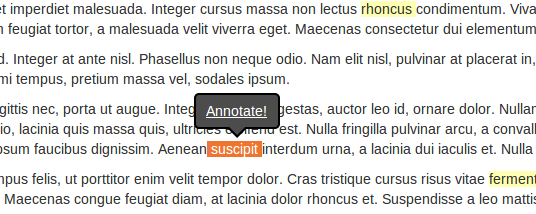
\includegraphics[width=.57\textwidth]{../PIC/annotate}\quad
  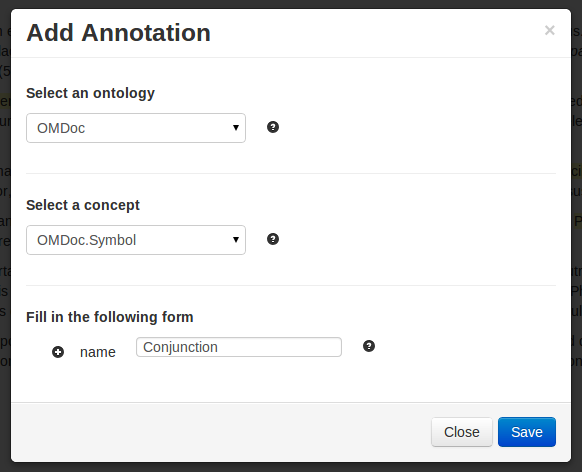
\includegraphics[width=.37\textwidth]{../PIC/add-symbol}
  \caption{Annotating in \KAT: Selection and Form-Filling}\label{fig:kat-annotate}
\end{figure}

\KAT is not tied to a particular annotation ontology (or ontology format). At startup, the
system is reads a set of \defemph{\KAT bindings} -- custom XML files that describe the
annotation interface, the constraints between the components of an annotation
frame\ednote{MK: I rather like this word for the relations you specify in one form; we
  should probably use it throughout. We should probably also rename ``concept'' to
  ``frame'' in the XML; I did that for the paper already.}, and the RDF to be
produced. The frame of OMDoc symbols used in Figure~\ref{fig:kat-annotate}, is given by
the fragment of a \KAT binding in Listing~\ref{lst:frame}. It specifies
\begin{inparaenum}[\em i\rm)]
\item the fields of the annotation form, their values and validation constraints,
\item their display, and
\item the RDF subgraph for the frame via a templating mechanism.
\end{inparaenum}
Note that this frame classifies the annotated word as an OMDoc symbol (via the \lstinline
[basicstyle=\sf\normalsize]|rdf:type| predicate) and relates it to its name via the
\lstinline[basicstyle=\sf\normalsize]|o:symbolname| relation from the OMDoc ontology.

\begin{lstlisting}[language=XML,label=lst:frame,
caption=A \KAT Frame Specification for OMDoc Symbols]
<frame name="Symbol">
    <help>An OpenMath/OMDoc Symbol</help>
    <fields>
        <field name="name" type="text">
            <help>The name of the symbol defines it in a theory</help>
            <value>Name</value>
            <default>Symbol</default>
            <validation>[A-Z][a-z]*</validation>
        </field>
    </fields>
    <display> ... </display>
    <rdf:RDF xmlns:rdf="http://www.w3.org/1999/02/22-rdf-syntax-ns#">
        <rdf:Description xmlns:o="http://omdoc.org/ontology#">
            <rdf:type rdf:resource="http://omdoc.org/ontology#Symbol"/>
            <o:symbolname>{name}</o:symbolname>
        </rdf:Description>
    </rdf:RDF>
</frame>
\end{lstlisting}
Even though \KAT can work as a standalone library that can be added to any STEM document
in HTML5, it is best used as a component of a corpus management system like the {Cor\TeX}
system~\cite{CorTeX:on} developed by the second author. In this situation the annotator
requests an annotation task from {Cor\TeX}, which serves the TEI-tokenized document with
\KAT and a set of bindings for the intended annotation ontologies. When the annotation is
complete, the generated RDF is exported to the semantic blackboard -- a RDF triple store
maintained by {Cor\TeX}. When combined with {Cor\TeX}, \KAT can be used by multiple
annotators; and can be used to review existing annotations, by importing them from the
triple store.  \KAT also has experimental support for inter-annotator agreement reviews
via a side-by-side view of the various annotations.

\section{Conclusion \& Future Work}\label{sec:concl}

We have presented the \KAT system, an open, parametric, and browser-based annotation
system for STEM documents encoded in HTML5.  The code released under the Gnu Public
License and is available at~\cite{KAT:github:on}. The system is in an early state of
development, but can already be used for practical annotation and annotation review work.
The user interface both needs and is yet to undergo serious usability testing and polish,
to both improve productivity and also to fully stabilize it for production use.
The next steps will be to refine our annotation ontologies and integrate more linguistic
ontologies to get more coverage. Also we want to start work on preparing a 
small annotated corpus of mathematical documents. 

\paragraph{Acknowledgements} Work on the concepts presented here has been partially
supported by the Leibniz association under grant SAW-2012-FIZ\_KA-2. We are grateful to
Goran Topi\'c from NII for discussions on the brat system.

\printbibliography
\end{document}

%%% Local Variables: 
%%% mode: latex
%%% TeX-master: t
%%% End: 

%  LocalWords:  StaKoh tlcspx10 ppte12 Rabe omdoc orga CorTeX localxscale localyscale lst
%  LocalWords:  tikzinput kat-arch Yawas yawas Annotatie annotatie nlex mathbb Wolska rdf
%  LocalWords:  DumGinKoh katsdm14 classificational kat-annotate includegraphics xmlns
%  LocalWords:  textwidth templating basicstyle normalsize symbolname lstlisting Cor
